


\section{Introduction}
\label{sec:intro}

The  French  state  has  been  facing severe  drought  events  over  the  past
decade. For instance,  the average annual cost of drought  events between 2016
and 2020  amounts to approximately  1.1 billion  EUROS, three times  more than
between 2002 and 2015. $\clubsuit$~citer swiss re~$\clubsuit$

France is  one of  the few  countries with  a system  that guarantees  all its
citizens adequate compensation in the event  of loss and/or damage caused by a
natural  phenomenon  such  as  severe  droughts.   The  compensation  scheme's
solidarity  is provided  by the  state-backed reinsurance  proposed by  Caisse
Centrale de Réassurance  (CCR), which enables the mutualisation  at a national
level of insurance portfolios and offers the State's guarantee.

Two prerequisites must be met to  trigger the compensation scheme.  First, the
lost  and/or damaged  property  must be  covered by  a  property and  casualty
insurance policy (a condition of  private nature). Second, a government decree
declaring a disaster must be published in the Official Journal (a condition of
public  nature).  It  is  the responsibility  of the  mayors  to initiate  the
request that  the government declare  a natural  disaster for the  cities they
administer.

At  the end  of each  civil  year, CCR  must  anticipate the  cost of  natural
disasters   that  occurred   during   the   year.   This   is   not  an   easy
task. \citet{osasl1,osasl2} developed  an algorithm to anticipate  the cost of
drought  events,  the  so-called   one-step  ahead  sequential  Super  Learner
(OSAS-SL).   Based on  the aggregation  of  a rich  library of  base-learners,
OSAS-SL  is  shown  to take  advantage  of  the  data  consisting of  a  short
time-series where  each time-specific observation  is a large network  of many
slightly  dependent data.   In their  application, the  authors consider  only
those  cities that  already benefit  from a  declaration of  natural disaster.
\citet{Charpentier_2021} also anticipate the  cost of drought events.  Simpler
than the OSAS-SL, their algorithm relies  on a generalized linear model and on
tree-based  machine learning  algorithms.   Unlike OSAS-SL,  it also  predicts
which cities will benefit eventually from a declaration of natural disaster.

In the present study, we focus on the prediction of requests of declaration of
natural disaster.  It  is a \textit{sparse prediction} task  because we expect
that  only  a  small  fraction  of  all French  cities  will  request  such  a
declaration.

\section{The data}
\label{sec:data}

The data  set is  obtained by merging  several data  sets.\footnote{Note that,
  from  now on,  France refers  to \textit{Metropolitan}  or \textit{Mainland}
  France.  Drought  events are  not a threat  in Overseas  France (essentially
  because there is little clay in these parts of the country).}

Given that we focus on drought events, it  will not come as a surprise that we
use the so-called  SWI (soil wetness index), an index  provided by MétéoFrance
(the French national meteorological service) that quantifies soil wetness in a
uniform  way,  see  \cite[][section~2.3]{Charpentier_2021} for  details.  More
specifically, for every  year and each city, the city-level  SWI is the convex
average of  the year-specific  SWIs of  the $8 \times  8$ km$^2$  squares that
overlap the  city's area.  The  weights are proportional  to the areas  of the
intersections.

The city-level  SWI is complemented with  data from other sources,  namely the
National  Institute   for  Statistical  and  Economic   Studies  (INSEE),  the
Geographic National Institute (IGN) and the French Geological Survey (BRGM).
% The new  features are city-specific  seismic hazard and climatic  zone, clay
% shrinkage-swelling hazards,  tree coverage rate, area,  population and years
% of construction.
Eventually,  for   every  year  and   each  city,  a   city-level  description
encapsulates  the  city's  profile.   The description  is  multi-faceted.   It
contains: an  indicator of whether or  not a natural disaster  was declared by
the government (when available); a summary  of the city's clay hazard, defined
as  the proportions  of houses  falling  in each  of four  categories of  clay
hazard; a  summary of the city's  dwelling age, \textit{i.e.}, how  old houses
are, under  the form  of the  proportions of  houses falling  in each  of four
categories;  the   climatic  and   seismic  zones   (a  five-category   and  a
four-category  variables); a  summary  of the  city's  vegetation; the  city's
number of houses, population, area,  average altitude, and density, defined as
the ratio  of the number  of houses  to the area.   In addition, a  variety of
features   are   described   by   quantiles   that   summarize   distributions
(\textit{e.g.},  the 30-quantiles  of the  distribution of  the house-specific
product of  SWI and insured value,  or the 30-quantile of  the distribution of
the house-specific product  of the ground slope and insured  value, to mention
just a  few).  Overall, the city-level  description consists of a  little more
than 430 variables.

\section{Some elements of optimal transport theory}
\label{sec:elements:OT}

The  methodology we  develop  to  make sparse  predictions  hinges on  optimal
transport theory.  This section presents the few tools that we will use.

Fix     arbitrarily    two     integers     $R,    R'     \geq    2$.      Let
$\bz := (z_{1}, \ldots, z_{R})$ and $\bz' := (z_{1}', \ldots, z_{R'}')$ be two
collections     of      elements     of     a     space      $\calZ$.      Let
$c : \calZ \times \calZ \to \bbR_{+}$ map any couple $(z,z')$ to a nonnegative
number interpreted as the cost to move  $z$ to $z'$, a cost function. The cost
function       $c$      induces       the       $R\times      R'$       matrix
$C(\bz,\bz')  \in \bbR_{+}^{R  \times R'}$  whose $(r,r')$-specific  component
$(C(\bz,\bz'))_{r,r'} := c(z_{r}, z_{r'}')$ is interpreted as the cost to move
$z_{r}$ to $z_{r'}'$ (relative to $c$).

Let
$\Pi_{R,R'}  := \{P  \in  \bbR_{+}^{R\times R'}  :  P\Ind_{R'} =  \tfrac{1}{R}
\Ind_{R},  P^{\top}\Ind_{R} =  \tfrac{1}{R'} \Ind_{R}\}$  represent the  joint
laws  on $\lb  R  \rb \times  \lb  R'\rb$ with  uniform  marginal laws,  where
$\lb  d \rb  :=  \{1, \ldots,  d\}$  for  every integer  $d\geq  1$. For  each
$P \in \Pi_{R,R'}$, let
\begin{equation*}
  E(P):= -\sum_{r\in  \lb R  \rb, r'  \in \lb R'  \rb} P_{r,r'}  \log P_{r,r'}
\end{equation*}
denote   the   entropy   of   $P$.   For  every   $P   \in   \Pi_{R,R'}$   and
$C \in \bbR_{+}^{R\times R'}$, let
\begin{equation*}
  \langle P,  C\rangle  := \sum_{r\in \lb  R \rb, r'  \in \lb  R' \rb}
  P_{r,r'} \times C_{r,r'}. 
\end{equation*}
When  $C  =  C(\bz,\bz')$,  $\langle   P,  C\rangle$  is  interpreted  as  the
$P$-specific cost to transport $\bz$ onto $\bz'$.

For any $\gamma > 0$ and $C \in \bbR_{+}^{R\times R'}$, introduce
\begin{equation}
  \label{eq:def:calW}
  \calW_{\gamma}(C)  :=  \min_{P   \in  \Pi_{R,R'}}  \left[\langle  P,
    C \rangle - \gamma E(P)\right].
\end{equation}
In particular,  when $C  = C(\bz,\bz')$, $\calW_{\gamma}(C(\bz,\bz'))$  is the
$\gamma$-regularized optimal cost to  transport $\bz$ onto $\bz'$, abbreviated
to ``the $\gamma$-regularized OT cost''.  Considering the $\gamma$-regularized
OT  cost   $\calW_{\gamma}(C(\bz,\bz'))$  instead  of  the   regular  OT  cost
$\calW_{0}(C(\bz,\bz'))$ (defined  as in~\eqref{eq:def:calW}  with $\gamma=0$)
has  two  important  merits~\cite[Chapters 3,  4,  9]{peyre2020computational}.
First,  $\bbR_{+}^{R\times R'}  \ni C  \mapsto \calW_{0}(C)  \in \bbR$  is not
differentiable                                                         whereas
$\bbR_{+}^{R\times   R'}  \ni   C\mapsto   \calW_{\gamma}(C)   \in  \bbR$   is
differentiable.   Second, for  any  $C \in  \bbR_{+}^{R\times R'}$,  computing
$\calW_{0}(C)$ requires  solving a costly  linear program via  network simplex
methods whereas  computing $\calW_{\gamma}(C)$ can be  performed easily thanks
to the so-called Sinkhorn algorithm~\cite{NIPS2013_af21d0c9}.

Finally,   we   use  the   $\gamma$-regularized   OT   cost  to   define   the
$\gamma$-regularized Sinkhorn cost
\begin{equation*}
  \calS_{\gamma}(\bz,\bz')       :=        \calW_{\gamma}(C(\bz,\bz'))       -
  \tfrac{1}{2}\left[\calW_{\gamma}(C(\bz,\bz))                               +
    \calW_{\gamma}(C(\bz',\bz'))\right]
\end{equation*}
(the  dependence of  $\calS_{\gamma}(\bz,\bz')$ on  the cost  function $c$  is
hidden).                         By~\citep[Theorem~1]{feydy2018interpolating},
$\calS_{\gamma} (\bz,\bz')  \geq \calS_{\gamma} (\bz,\bz) =  0$.  Moreover, we
stress that $\calS_{\gamma} (\bz,\bz')$ can be computed with little additional
computational cost compared to $\calW_{\gamma} (\bz,\bz')$.


\section{Making sparse predictions}
\label{sec:sparse:regression}

$\clubsuit$~dire  que c'est  sans doute  très  difficile de  procéder via  des
prédicteurs, pour plusieurs raisons:
\begin{itemize}
\item pas évident de prendre la contrainte de parcimonie en compte;
\item difficile de trouver les bonnes covariables;
\item en lien avec  la difficulté ci-dessus, il est plus  naturel de penser en
  termes de comparaisons deux à deux;
\item  hypothèse  de  stationnarité  (de  la  loi  de  $Y$  sachant  $X$)  pas
  évidente\ldots 
\end{itemize}

\subsection{Translation to an optimization problem}
\label{subsec:opt:pbm}

We denote  by $x_{m}  \in\calX$ ($m  \in \lb M  \rb$) the  $m$th year-specific
city-level description for which it is known whether or not the city requested
a declaration of natural disaster for  a drought event, a piece of information
denoted  by $y_{m}  \in\{0,1\}$ (with  convention $y_{m}=1$  if the  city with
year-specific city-level  description $x_{m}$  did request such  a declaration
that year).  Moreover, we denote by $x_{n}'\in  \calX$ ($n \in \lb N \rb$) the
$n$th year-specific city-level description for  which it is \textit{not} known
whether  or  not the  city  \textit{will}  request  a declaration  of  natural
disaster for  a drought event.  Predicting  for each of the  cities whether or
not that will be the case is our objective.


To do so, we propose to solve the following optimization problem:
\begin{equation}
  \label{eq:main:pbm}
  \mathop{\arg\min}_{\theta    \in     \bbR^{N}}    \left\{\calS_{\gamma}(\bz,
    \bz'(\theta)) + g_{\tau}(\theta) \right\}, 
\end{equation}
where
\begin{itemize}
\item for all $\theta \in \bbR^{N}$,
  \begin{equation*}   \bz    :=   \left((x_{1},   y_{1}),    \ldots,   (x_{M},
      y_{M})\right), \quad \bz'(\theta) := \left((x_{1}', \theta_{1}), \ldots,
      (x_{N}', \theta_{N})\right);
  \end{equation*}
\item                   the                    cost                   function
  $c : (\calX \times \bbR)\times (\calX \times \bbR)\to \bbR_{+}$ is given by
  \begin{equation*}
    c\left((x,y), (x', \theta)\right) := \dis(x,x')^{2} + (y - \theta)^{2} 
  \end{equation*}
  for a distance or dissimilarity $\dis$ on $\calX$;
\item    $g_{\tau}$    is    a     convex    function    given    by    either
  $g_{\tau}(\theta)  := \|\theta\|_{1}  + \II\{\theta  \in [0,1]^{N}\}$,  with
  $\|\theta\|_{1}:=    \sum_{n   \in    \lb   N    \rb}   |\theta_{n}|$,    or
  $g_{\tau}(\theta)  :=  \II\{\|\theta\|_{1}  \leq \tau\}  +  \II\{\theta  \in
  [0,1]^{N}\}$,  where  $\II\{A\}$ equals  0  if  $A$  is true  and  $+\infty$
  otherwise;
\item $\gamma, \tau > 0$ are some user-supplied constants.
\end{itemize}
 

A few comments are in order.
\begin{enumerate}
\item  The  argmin  in  \eqref{eq:main:pbm}   is  over  $\bbR^{N}$  but  could
  equivalently     be    over     $[0,1]^{N}$     (even     if    the     term
  $\II\{\theta  \in   [0,1]^{N}\}$  was   dropped  from  the   definitions  of
  $g_{\tau}(\theta)$).  We thus view $\theta_{n}$  as the probability that the
  city described  by $x_{n}'$ will  request a declaration of  natural disaster
  for a drought event.
\item $\clubsuit$~parler ici du rôle-clef de la matrice $C(\theta)$?\ldots
\item For  both choices of  $g_{\tau}$, the  $\ell^{1}$-norm of $\theta$  is a
  substitute for $\card\{n \in \lb N \rb : \theta_{n} \neq 0\}$.
\item  Adding  the  penalization   term  $+  g_{\tau}(\theta)$  favors  sparse
  solutions, which  is in line  with our  prior knowledge that  relatively few
  cities will eventually indeed request  a declaration of natural disaster for
  a drought event.

  The                                case                                where
  $g_{\tau}  (\theta)  =  \II\{\|\theta\|_{1}\leq  \tau\}  +  \II\{\theta  \in
  [0,1]^{N}\}$  is quite  interesting  since  it is  easier  to fine-tune  the
  parameter $\tau$,  especially because  experts at CCR  may sometimes  have a
  rough idea of how many cities will request a declaration of natural disaster
  for a drought event.
\end{enumerate}

\subsection{On solving \textbf{\eqref{eq:main:pbm}}}
\label{subsec:solving}

Solving \eqref{eq:main:pbm}  is not straightforward, because  the criterion to
minimize   is   the   sum    of   the   non-convex   differentiable   function
$f:\theta\mapsto      \calS_{\gamma}       (\bz,      \bz'(\theta))$      (see
Section~\ref{subsubsec:f:smooth})   and  of   the  convex   non-differentiable
function  $g_{\tau}$.    Luckily,  we  can   rely  on  the   so-called  iPiano
algorithm~\cite{iPiano}  which  was  developed  precisely to  deal  with  such
optimization problems.

The       iPiano       algorithm       starts      from       an       initial
$\theta^{-1}  = \theta^{0}  \in ]0,1[^{N}$  and the  update scheme  informally
writes as (below, $\alpha,\beta$ are positive constants)
\begin{equation}
  \theta^{k+1} = \Prox_{\alpha g_{\tau}} \left(\theta^k - \alpha \nabla f(\theta^k) +
    \beta (\theta^k - \theta^{k-1}) \right), 
\end{equation}
where the proximal map $\Prox_{\alpha g_{\tau}}$ is defined by
\begin{equation}
  \label{eq:proximal:map}
  \Prox_{\alpha  g_{\tau}}   (t)  :=  \mathop{\arg\min}_{\theta   \in  \bbR^N}
  \left\{\tfrac{1}{2}\|\theta-t\|_2^2 + \alpha g_{\tau}(\theta)\right\}.  
\end{equation}
On                the                one               hand,                if
$g_{\tau} (\theta) =  \tau \|\theta\|_{1} + \II\{\theta  \in [0,1]^{N}\}$ then
\eqref{eq:proximal:map} is simply given by
\begin{equation*}
  \left(\Prox_{\alpha g_{\tau}} (t)\right)_{n} = \min\{\left(|t_{n}| -
    \alpha\tau\right)_{+}, 1\}.  
\end{equation*}
In       particular,        if       $t       \in        [0,1]^{N}$       then
$(\Prox_{\alpha g_{\tau}} (t))_{n} =  \left(t_{n} - \alpha\tau\right)_{+}$ for
every     $n    \in     \lb    N\rb$.      On    the     other    hand,     if
$g_{\tau}  (\theta)  =  \II\{\|\theta\|_{1}  \leq  \tau\}  +  \II\{\theta  \in
[0,1]^{N}\}$  then the  proximal  map  is the  Euclidean  projection onto  the
$\ell^{1}$-ball centered at 0 and  with radius $\tau$.  An efficient algorithm
is available to implement this projection~\cite{L1-ball}.

Moreover,   following~\cite[Section   4.3]{pmlr-v32-cuturi14},  we   show   in
Section~\ref{subsubsec:f:smooth} that the gradient of $f$ is given by
\begin{align}
  \notag
  \nabla f(\theta)
  &  =  \nabla  \calW_{\gamma}  (C(\bz, \bz'(\theta))  -  \tfrac{1}{2}  \nabla
    \calW_{\gamma} \left(C(\bz'(\theta), \bz'(\theta))\right) \\
  \notag
  &    =    2(\tfrac{1}{N}\theta    -   \widehat{P}_{\theta}^{\top}    y)    -
    (\tfrac{2}{N}\theta - (\widehat{Q}_{\theta} + \widehat{Q}_{\theta}^{\top})
    \theta)\\
  \label{eq:gradient:f}
  &   =   -2   \widehat{P}_{\theta}^{\top}   y   +   (\widehat{Q}_{\theta}   +
    \widehat{Q}_{\theta}^{\top} )    \theta
\end{align}
with
\begin{align}
  \label{eq:hatPtheta}
  \widehat{P}_{\theta} 
  & = \mathop{\arg\min}_{P \in \Pi_{M,N}}
    \left\{\langle P, C(\bz,\bz'(\theta)) \rangle - \gamma E(P)\right\},\\ 
  \label{eq:hatQtheta}
  \widehat{Q}_{\theta} 
  & = \mathop{\arg\min}_{P \in \Pi_{N,N}}
    \left\{\langle   P,  C(\bz'(\theta),   \bz'(\theta))   \rangle  -   \gamma
    E(P)\right\}. 
\end{align}

We check that the assumptions  of \cite[Theorems~4.9 and 4.14]{iPiano} are met
by  proving that  $f$  is  $C^{1}$-smooth with  an  $L$-Lipschitz gradient  on
$\dom  g_{\tau}$ and  that  $(f+g_{\tau})$  satisfies the  Kurdyka-Lojasiewicz
property on its  domain (the proof is  presented in Section~\ref{sec:iPiano}).
Therefore we can assert that
\begin{itemize}
\item the sequence $(\theta^{k})_{k \geq 0}$  converges to a critical point of
  $\theta \mapsto f(\theta) + g_{\tau}(\theta)$;
\item $\min_{k \leq K} \|\theta^{k+1} - \theta^{k}\|_{2}^{2} = O(K^{-1})$;
\item                      if                      we                      set
  $r(\theta)  :=  \theta  -  \Prox_{\alpha g_{\tau}}  (\theta  -  \alpha\nabla
  f(\theta))$, then $\min_{k \leq K} \|r(\theta^{k})\|_{2}^{2} = O(K^{-1})$.
\end{itemize}
The   so-called  proximal   residual   $r(\theta)$   is  interesting   because
$r(\theta) =  0$ means  that the  first-order optimality  condition is  met at
$\theta$.  Indeed (denoting by $\partial  \ell (x)$ either the subdifferential
of the  convex function~$\ell$ at  $x$ or the limiting-subdifferential  of the
proper    lower     semicontinuous    function    $\ell$    at     $x$,    see
Section~\ref{subsubsec:KL}), $r(\theta) = 0$ if and only if (iff)
\begin{align*}
  \theta = \Prox_{\alpha g_{\tau}} (\theta - \theta \nabla f(\theta))
  & \quad\text{iff}\quad  0 \in \partial \left(\tfrac{1}{2} \|\theta - \alpha \nabla
    f(\theta)       -      \cdot\|_{2}^{2}       +      \alpha
    g_{\tau}\right)(\theta) \\
  & \quad\text{iff}\quad 0 \in \{\theta - (\theta - \alpha \nabla f(\theta))\} +
    \alpha \partial g_{\tau}(\theta)\\
  & \quad\text{iff}\quad 0  \in \{\alpha \nabla f(\theta)\}  + \alpha \partial
    g_{\tau}(\theta) \\
  & \quad\text{iff}\quad 0 \in \partial(f + g_{\tau})(\theta).
\end{align*}

\section{Implementation}
\label{sec:implementation}

$\clubsuit$~We  already  wrote  a \texttt{python}/\texttt{pytorch}  script  to
solve \eqref{eq:main:pbm}; \textcolor{red}{using \texttt{geomloss} and \texttt{MissingDataOT} modules}  and we are  currently preparing the application.  We
will illustrate and comment on our results.

Carrying out the application is not easy. This is notably because \textit{(i)}
$M$ and  $N$ are  large ($M\approx  20 \times  36000 =  72 \times  10^{4}$ and
$N \approx 36000$)  and \textit{(ii)} $\calX$ is a  high-dimensional space and
the choice  of the distance/dissimilarity $d$  on $\calX$ is difficult.   As a
consequence,  we have  to  rely  on a  mini-batch  procedure  to evaluate  the
gradient of $f$. This poses both computational and theoretical challenges.


\section{A simple simulation study}
\label{sec:simul}

We conduct a simulation study to illustrate our procedure in a simple context.

\subsection{Simulation scheme}
\label{subsec:sim:scheme}

For any $p\in(0,1)$, let $P_{p}$ be  the law on $\bbR^{2} \times \{0,1\}$ such
that
\begin{itemize}
\item if $R$  and $\alpha$ are independently drawn from  the $\chi^{2}(1)$ law
  % (the $\chi^{2}$ law with one degree of freedom)
  and      from      the      uniform     law      on      $[0,2\pi]$,      if
  $X =  (R\cos(\alpha), R\sin(\alpha))$ and  if, conditionally on $X$,  $Y$ is
  drawn from  the Bernoulli law  with parameter  $\expit(c(p) + R)$,  then the
  joint law of $(X,Y)$ is $P_{p}$;
\item  the above  constant  $c(p) \in  \bbR$  is  chosen in  such  a way  that
  $E_{P}(Y) = P(Y=1) = p$.
\end{itemize}
For   instance,  $c(20\%)   \approx  -2.64$,   $c(10\%)  \approx   -3.83$  and
$c(5\%) \approx  -5.00$.  Note that,  for any $p\in(0,1)$, under  $P_{p}$, the
further $X$ is from 0 the more likely it is that $Y=1$.

For each $p\in\{20\%, 10\%,5\%\}$, we independently sample $n=100$ independent
copies   of  $(X,Y)$   under   $P_{p}$.   We   thus   obtain  $M=3n$   couples
$(x_{m}, y_{m})$.  Moreover, we  also sample independently $n=100$ independent
copies of  $(X,Y)$ from the law  $P_{p}$ with $p=10\%$.  We  thus obtain $N=n$
couples  $(x_{n}',y_{n}')$.  In  this simulation  study, our  objective is  to
recover    the    vector    $(y_{n}')_{n    \in   \lb    N\rb}$    based    on
$\{(x_{m}, y_{m}) : m \in \lb M\rb\}$ and on $(x_{n}')_{n \in \lb N\rb}$.

\subsection{Fine-tuning our procedure}

Let  us first  describe how  we fine-tune  our procedure  in order  to predict
$(y_{n}')_{n \in \lb  N\rb}$ by solving \eqref{eq:main:pbm}. On  the one hand,
we choose the dissimilarity on $\bbR^{2}$ given by
\begin{equation*}
  \dis(x,x')^{2}:= \left|\sqrt{x_{1}^{2} + x_{2}^{2}} - \sqrt{(x_{1}')^{2} + 
      (x_{2}')^{2}}\right|.
\end{equation*}
Admittedly, this puts us in a  favorable position because the true conditional
probability   of    the   event    $Y=1$   given    $X$   only    depends   on
$\sqrt{X_{1}^{2} +  X_{2}^{2}}$.  On  the other hand,  we choose  the function
$g_{\tau}  : \theta  \mapsto \II\{\|\theta\|_{1}  \leq 5\}  + \II\{\theta  \in
[0,1]^{N}\}$.   Note  that $\sum_{n  \in  \lb  N\rb}  y_{n}'$ (the  number  of
$y_{n}'$s equal to  1) can be viewed  as the realization of  a random variable
$S$ drawn from the binomial law with  parameter $(100, 10\%)$. The mean of $S$
equals 10 and $S$ falls in $[5, 15]$ with probability larger than $93\%$. This
second fact motivates the choice of $\tau=5$ in the definition of $g_{\tau}$.

$\clubsuit$~que   dire    de   plus   des    choix   que   l'on    fait?    Cf
Section~\ref{sec:implementation}

\subsection{Alternative, classification-based approaches}

As  an alternative  approach  to  predicting $(y_{n}')_{n  \in  \lb N\rb}$  by
solving  \eqref{eq:main:pbm}, we  also  consider training  an algorithm  using
$\{(x_{m}, y_{m})  : m  \in \lb  M\rb\}$ in  order to  learn to  classify each
$x_{n}'$ individually.  Instead  of selecting one algorithm, we  rely on super
learning  to  learn  and  train  a meta-algorithm  that  builds  upon  several
algorithms to classify at least as well as (and sometimes better than) all the
candidate                   algorithms~\citep[and                   references
therein]{SL2007,SuperLearner,SLchapter}. We choose  four individual algorithms
to  learn  the conditional  probability  of  the  event  $Y=1$ given  $X$:  an
algorithm that approximates it under the form of a constant function (in $X$);
an   algorithm   that   learns   which    element   of   the   working   model
$\{x \mapsto  \expit(t_{0} + t_{1}  x_{1} + t_{2}  x_{2}) : t  \in \bbR^{3}\}$
best approximates it  (\texttt{glm}); an algorithm that  approximates it under
the form of a tree, using  the covariates $X_{1}$ and $X_{2}$ (\texttt{rpart},
\citet{rpart}); an algorithm  that approximates it under the form  of a random
forest,   using  the   covariates   $X_{1}$   and  $X_{2}$   (\texttt{ranger},
\citet{ranger}). 

In  addition, we  consider  a second  super learning  procedure  to learn  the
conditional  probability of  the  event  $Y=1$ given  $X$  by  relying on:  an
algorithm that approximates it under the form of a constant function (in $X$);
an   algorithm   that   learns   which    element   of   the   working   model
$\{x \mapsto \expit(t_{0} + t_{1} x_{1}  + t_{2} x_{2} + t_{3} \sqrt{x_{1}^{2}
  + x_{2}^{2}})  : t \in  \bbR^{4}\}$ best approximates it  (\texttt{glm}); an
algorithm that approximates it under the  form of a tree, using the covariates
$X_{1}$, $X_{2}$ and  $\sqrt{X_{1}^{2} + X_{2}^{2}} =  R$ (\texttt{rpart}); an
algorithm that  approximates it under the  form of a random  forest, using the
covariates $X_{1}$,  $X_{2}$ and $R$  (\texttt{ranger}). We expect  the second
super learner  to perform  better than the  first one because  it can  use the
relevant covariate $R$.

$\clubsuit$~à reprendre\ldots

\begin{figure}
  \centering
  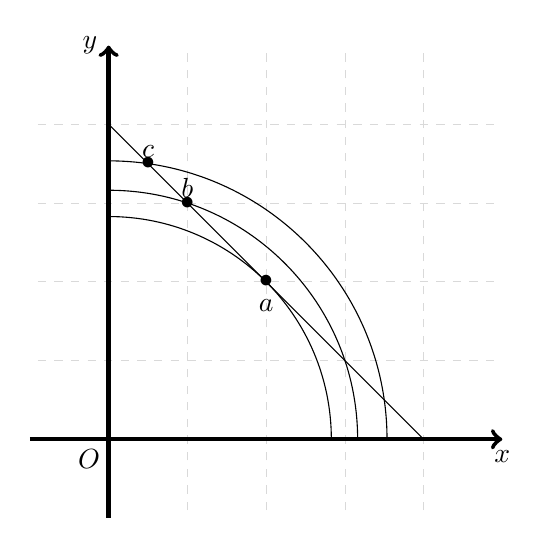
\begin{tikzpicture}
    \draw[help lines, color=gray!30, dashed] (-0.9,-0.9) grid (4.9,4.9);
    % 
    \draw[->,ultra thick] (-1,0)--(5,0) node[below]{$x$};
    % 
    \draw[->,ultra thick] (0,-1)--(0,5) node[left]{$y$};
    % 
    \draw[-] (0,4)--(4,0);
    %
    \node (O) at (-0.25,-0.25) {$O$};
    %%%%%%%%%%%%%%%%%%%%%% 
    \pgfmathparse{sqrt(0.5^2+3.5^2)};
    % 
    \node[label={[shift={(0,-0.25)}]$c$}] (C) at (0.5,3.5) {$\bullet$};
    % 
    \node (C) at (0,\pgfmathresult) {};
    % 
    \draw (C) arc[start angle=90, end angle=0, radius=\pgfmathresult];
    %%%%%%%%%%%%%%%%%%%%%% 
    \pgfmathparse{2*sqrt(2)};
    % 
    \node[label={[shift={(0,-0.7)}]$a$}] (A) at (2,2) {$\bullet$};
    % 
    \node (A) at (0,\pgfmathresult) {};
    % 
    \draw (A) arc[start angle=90, end angle=0, radius=\pgfmathresult];
    %%%%%%%%%%%%%%%%%%%%%% 
    \pgfmathparse{sqrt(10)};
    % 
    \node[label={[shift={(0,-0.25)}]$b$}] (B) at (1,3) {$\bullet$};
    % 
    \node (B) at (0,\pgfmathresult) {};
    % 
    \draw (B) arc[start angle=90, end angle=0, radius=\pgfmathresult];
  \end{tikzpicture}
  \label{fig:explain}
  \caption{The      segment      represents      (in     2D)      the      set
    $S_{a}:=\{u \in  (\bbR_{+})^{d} :  \|u\|_{1} = \|a\|_{1}\}$.   It contains
    $a,b,c$.   The  circles  are  centered  at  the  origin  and  have  radius
    $\|a\|_{2}$ or $\|b\|_{2}$ or $\|c\|_{2}$.   For any $v \in S_{a}$, define
    $R_{v}:= \{u \in (\bbR_{+})^{d} :  \|u\|_{1} \geq \|v\|_{1} \geq \|v\|_{2}
    \geq     \|u\|_{2}\}$.      Then,      for     all     $v,w\in     S_{a}$,
    $\|v-a\|_{2} \leq \|w-a\|_{2}$ implies $R_{v} \subset R_{w}$.}
\end{figure}

\section{Application}
\label{sec:appli}


\section{Discussion}
\label{sec:discussion}

\section{Proof: Checking the iPiano assumptions}
\label{sec:iPiano}

The iPiano assumptions consist in 
\begin{enumerate}
\item  $f$  being  $C^{1}$-smooth  with a  Lipschitz  continuous  gradient  on
  $\dom g_{\tau}$, see Section~\ref{subsec:assum:f};
\item for  any $\delta >  0$, $H_{\delta} :  \bbR^N \times \bbR^{N}  \to \bbR$
  given                                                                     by
  $H_{\delta} (\theta,  \theta') := f(\theta')  + g_{\tau} (\theta')  + \delta
  \|\theta -  \theta'\|_{2}^{2}$ having the Kurdyka-Lojasiewicz  property at a
  cluster   point   $(\theta^{\star},   \theta^{\star})$   of   the   sequence
  $(\theta^{k})_{k \geq 1}$, see Section~\ref{subsec:KL}.
\end{enumerate}



\subsection{The function  \boldmath{$f$} is  \boldmath{$C^{1}$}-smooth and
  its gradient is Lipschitz continuous on \boldmath{$\dom g_{\tau}$}}
\label{subsec:assum:f}

\subsubsection{Preliminaries}

\paragraph{On matrix norms.}


For  self-containedness,  let  us   recall  several  definitions  and  results
concerning  matrix norms.   For  any  matrix $A  \in  \bbR^{d\times d'}$,  the
Frobenius     and     maximum     norms     of    $A$     are     given     by
$\|A\|_F :=  \left(\sum_{i \in  \lb d \rb,  j \in  \lb d'
    \rb}                   A_{i,j}^2\right)^{1/2}$                  and
$\|A\|_{\max}  := \max  \{|A_{i,j}| :  i \in  \lb d  \rb, j  \in
\lb d'  \rb\} $.  For any  vector $x \in \bbR^d$,  the variation
seminorm           of           $x$          is           defined           as
$\|x\|_{\var} := \max \{x_{i} : i\in \lb d \rb \} - \min \{x_{i}
:  i \in  \lb d  \rb\}$.  We  will use  the following  classical
inequalities and equality:
\begin{align}
  \label{eq:ineq1}
  \forall  A\in  \bbR^{d \times  d'},  \forall  B  \in \bbR^{d'  \times  d''},
  \|AB\|_F \leq  \|A\|_F \|B\|_F;\\
  \label{eq:ineq2}
  \forall A  \in \bbR^{d \times  d'}, \forall  x \in \bbR^{d'},  \|Ax\|_2 \leq
  \|A\|_F \|x\|_2;\\
  \label{eq:ineq3}
  \forall x \in \bbR^{d}, \|\diag(x)\|_F = \|x\|_2;\\
  \label{eq:ineq44}
  \forall x \in \bbR^{d}, \|x\|_{\var} \leq 2 \|x\|_{\infty};\\
  \label{eq:ineq55}
  \forall x \in \{0\} \times \bbR^{d-1}, \|x\|_{\infty} \leq \|x\|_{\var}. 
\end{align}
\paragraph{On the Hilbert projective metric.}

The Hilbert projective metric on $(\bbR_{+}^{*})^{d}$ is defined by
\begin{equation*}
  \forall x, x' \in  (\bbR_{+}^{*})^{d}, d_{\calH}
  (x,x') :=  \log \max\left\{\tfrac{x_i x'_j}{x'_i  x_j} : i,j \in  \lb d
    \rb\right\}.
\end{equation*}
We will use the following properties~\cite{Birkhoff}:
\begin{gather}
  \label{eq:ineq4}
  \forall x, x' \in (\bbR_{+}^{*})^{d}, d_{\calH} (x,x') = \| \log(x) -
  \log(x') \|_{\var};\\
  \label{eq:ineq5}
  \forall x, x' \in (\bbR^{*}_{+})^{d}, d_{\calH}(x, x') = d_{\calH}(x/x',
  \Ind_d) = d_{\calH}(\Ind_d/x', \Ind_d/x);\\
  \label{eq:ineq6}
  \forall K \in (\bbR_{+}^{*})^{d \times d'}, \forall x, x' \in
  (\bbR^{*}_{+})^{d'}, d_{\calH}(Kx, Kx') \leq \lambda(K) d_{\calH}(x, x'),
\end{gather}
where  $\lambda(K) :=  \tfrac{\sqrt{\eta(K)} -1}{\sqrt{\eta(K)}+1}  < 1$  with
$\eta(K) :=  \max\left\{\tfrac{K_{i,k} K_{j,\ell}}{K_{j,k} K_{i, \ell}}  : i,j
  \in \lb d \rb, k,\ell \in \lb d' \rb\right\}$. 

We end this section with a lemma.
\begin{lemma}
  \label{lem:inq:norm}
  Let     $x,      x'     \in      (\bbR_{+}^{*})^d$     be      such     that
  $0  < t  \leq \min\{x_{j},  x_{j}' :  j \in  \lb d  \rb\} \leq
  \max\{x_{j}, x_{j}'  : j \in  \lb d  \rb\} \leq T$.   It holds
  that  $\tfrac{1}{2}t  d_{\calH}(x,  x') \leq  \|x-x'\|_{2}$.   Moreover,  if
  $x_1     =     x'_1     =     1$,    then     it     also     holds     that
  $\|x-x'\|_{2} \leq \sqrt{d}T d_{\calH}(x, x')$.
\end{lemma}
\begin{proof}
  % For all $q \in \bbR$, $e^q \geq 1 +q$.  If $q \geq 0$ then
  % $ e^q -1\geq q \geq 0$ so it implies $|e^q-1| \geq |q|$.  If $q \leq 0$
  % then $-q \geq 1-e^q \geq 0$ hence it implies that $|q| \geq |1-e^q|$.\\
  Set  $x, x'  \in (\bbR_{+}^{*})^d$  as in  the statement  of the  lemma, and
  denote   $\ell:=   \log(x),  \ell'   :=   \log(x')$   (the  logarithms   are
  elementwise). Set arbitrarily $i \in \lb  d \rb$. We can assume without loss
  of    generality   that    $x_{i}    \geq    x_{i}'$   (or,    equivalently,
  $\ell_{i}  \geq   \ell_{i}'$).   Therefore   if  $x_{1}  =   x_{1}'=1$  (or,
  equivalently, $\ell_{1} = \ell_{1}' = 0$), then
  \begin{align*}
    |x_i - x'_i |&= \max(x_i, x'_i) \times |1 - e^{-|\ell_i- \ell'_i|}|\\
                 &\leq T \times |\ell_i- \ell'_i| \quad \text{ because }
                   |1-e^{-|q|}| \leq |q| \text{ for all } q \in \bbR\\
                 &\leq T \times \|\ell- \ell'\|_{\infty} \\
                 &\leq   T   \times  \|\ell-
                   \ell'\|_{\var} \quad \text{by \eqref{eq:ineq55} since }\ell_{1} =
                   \ell_{1}' = 0\\
                 &= T d_{\calH}(x, x') \quad \text{by \eqref{eq:ineq4}}. 
  \end{align*}
  Consequently,
  $\|x -x'\|_{2} \leq \sqrt{d} \|x -x'\|_{\infty} \leq \sqrt{d} T d_{\calH}(x,
  x')$.  Furthermore,
  \begin{align*}
    |x_i- x'_i |&= \min(x_i, x'_i) \times |e^{|\ell_i- \ell'_i|} -1|\\
                & \geq t \times |\ell_i- \ell'_i| \quad \text{ because }
                  |e^{|q|} - 1| \geq |q| \text{ for all } q \in \bbR.
  \end{align*}
  It follows that
  \begin{align*}
    \|x -x'\|_{2} \geq\|x -x'\|_{\infty} \geq t \|\ell- \ell'\|_{\infty}
    & \geq \tfrac{1}{2}t \|\ell- \ell'\|_{\var} \quad \text{by \eqref{eq:ineq44}}\\
    &=  \tfrac{1}{2}td_{\calH}(x, x') \quad \text{by \eqref{eq:ineq4}}.
  \end{align*}
  This completes the proof.
\end{proof}

\subsubsection{The function $f$ is differentiable}
\label{subsubsec:f:smooth}

To  prove that  $f$  is differentiable,  we rely  on  the following  classical
result~\cite{Danskin}:
\begin{theorem}[Danskin's theorem, Proposition~B.25 in \cite{Bertsekas99}]
  Let    $\calC     \subset    \bbR^{d'}$    be    a     compact    set    and
  $\phi: \bbR^{d} \times \calC \rightarrow \bbR$ be a continuous function such
  that  $\phi(\cdot, y)$  is convex  for every  $y \in  \calC$.  The  function
  $\psi:\bbR^{d} \to \bbR$ given by $\psi(x) := \max_{y \in \calC} \phi(x, y)$
  is  convex.   Moreover,  if  there  exists  a  unique  $\hat{y}$  maximizing
  $\phi(x,  \cdot)$  and if  $\phi(\cdot,  \hat{y})$  is differentiable,  then
  $\psi$         is         differentiable          at         $x$         and
  $\nabla \psi(x) = \nabla \phi(\cdot, \hat{y})|_{x}$.
\end{theorem}
Let      $\calC      =      \Pi_{R,R'}$     (a      compact      set)      and
$\phi:\bbR^{R\times   R'}   \times   \Pi_{R,R'}   \to  \bbR$   be   given   by
$\phi(C,P) := -[\langle P, C \rangle  - \gamma E(P)]$.  The function~$\phi$ is
continuous  and $\phi(\cdot,  P)$  is  convex for  every  $P \in  \Pi_{R,R'}$.
Therefore,       by      the       above      theorem,       the      function
$\psi     :     \bbR^{R     \times      R'}     \to     \bbR$     given     by
$\psi(C)  :=  \max_{P \in  \Pi_{R,R'}}  \phi(C,P)  = -\calW_{\gamma}  (C)$  is
convex. Moreover, for every $C \in  \bbR^{R \times R'}$, there exists a unique
$\widehat{P}_{C}$                           such                          that
$\psi(C) = \phi(C, \widehat{P}_{C})$~\cite[Proposition 4.3]{pmlr-v32-cuturi14}
and $\phi(\cdot, \widehat{P}_{C})$ is affine hence differentiable.  Therefore,
$C\mapsto      \calW_{\gamma}(C)$     is      differentiable     at      every
$C    \in    \bbR^{R    \times    R'}$    with    a    gradient    given    by
$\nabla\calW_{\gamma}(C) = \widehat{P}_{C}$.

We  use now  that  $f  = f_{a}  -  \tfrac{1}{2}f_{b}  + \text{constant}$  with
$f_{a},f_{b} : \bbR^{N} \to \bbR$ given by
\begin{equation*}
  f_{a}(\theta)   :=  \calW_{\gamma}   \left(C(\bz,\bz'(\theta))\right)  \quad
  \text{and}        \quad        f_{b}(\theta)        :=        \calW_{\gamma}
  \left(C(\bz'(\theta),\bz'(\theta))\right) 
\end{equation*}
where       the       cost      matrices       $C(\bz,\bz'(\theta))$       and
$C(\bz'(\theta),\bz'(\theta))$            are             such            that
$(C(\bz,\bz'(\theta)))_{m,n}   :=   \dis(x_{m},   x_{n}')^{2}   +   (y_{m}   -
\theta_{n})^{2}$                                                           and
$(C(\bz'(\theta),\bz'(\theta)))_{n,n'}   :=    \dis(x_{n}',   x_{n'}')^{2}   +
(\theta_{n} -  \theta_{n'})^{2}$.  In view  of the previous paragraph,  and by
the  chain  rule,  $f_{a}$  and  $f_{b}$  are  thus  differentiable  at  every
$\theta \in \bbR^{N}$ with gradients
% \begin{align*}
%   \nabla f_{a}(\theta)
%   & = \left(2\sum_{m=1}^{M} (\widehat{P}_{\theta})_{m,n} 
%     (\theta_{n} - y_{m})\right)_{n=1}^{N} =
%     2 (\tfrac{1}{N}\theta - \widehat{P}_{\theta}^{\top} y),\\ 
%   \nabla f_{b}(\theta)
%   & =   2   (\tfrac{2}{N}\theta   -
%     (\widehat{Q}_{\theta} + \widehat{Q}_{\theta}^{\top}) y)\\ 
% \end{align*}
\begin{equation*}
  \nabla f_{a}(\theta)  = 2 (\tfrac{1}{N}\theta  - \widehat{P}_{\theta}^{\top}
  y) \quad \text{and} \quad 
  \nabla  f_{b}(\theta)  =  2 (\tfrac{2}{N}\theta  -  (\widehat{Q}_{\theta}  +
  \widehat{Q}_{\theta}^{\top}) \theta)
\end{equation*}
($\widehat{P}_{\theta}$     and     $\widehat{Q}_{\theta}$     are     defined
in~\eqref{eq:hatPtheta}   and   \eqref{eq:hatQtheta}).    Therefore   $f$   is
differentiable  at  every  $\theta  \in  \bbR^{N}$  and  \eqref{eq:gradient:f}
follows straightforwardly.

\subsubsection{ $\widehat{P}_{\theta}$                           and
  $\widehat{Q}_{\theta}$ are Lipschitz  continuous (as functions of
  $\theta$)}
\label{subsec:phat:qhat:lipschitz}

The     fact     that     $\theta    \mapsto     \widehat{P}_{\theta}$     and
$\theta\mapsto    \widehat{Q}_{\theta}$    are   Lipschitz    continuous    on
$\dom g_{\tau}$ is a consequence of the following lemma.
\begin{lemma}
  \label{lem:phat}
  Let  $\theta  \mapsto  C(\theta)$  be a  bounded  and  Lipschitz  continuous
  function   from  $[0,1]^{R'}$   to   $\bbR_{+}^{R\times   R'}$.   For   each
  $\theta\in[0,1]^{R'}$,  let   $\widehat{P}(\theta)$  be  the   minimizer  in
  \eqref{eq:def:calW}   with   $C(\theta)$    substituted   for   $C$.    Then
  $\theta   \mapsto   \widehat{P}(\theta)$   is  Lipschitz   continuous   from
  $[0,1]^{R'}$ to $\bbR_{+}^{R\times R'}$.
\end{lemma}
\noindent      Indeed,       $\theta\mapsto      C(\bz,\bz'(\theta))$      and
$\theta\mapsto        C(\bz'(\theta),\bz'(\theta))$         (defined        in
Section~\ref{subsubsec:f:smooth})   are   obviously  bounded   and   Lipschitz
continuous.

Let       us      prove       Lemma~\ref{lem:phat}.       By~\cite[Proposition
4.3]{pmlr-v32-cuturi14}, for every $\theta \in \bbR^{R'}$,
\begin{align*}
  \widehat{P}(\theta)
  & = \diag(\widehat{u}(\theta)) K(\theta)
    \diag(\widehat{v}(\theta)),
\end{align*}
where    $\widehat{u}    :    \bbR^{R'}    \rightarrow    (\bbR_{+}^{*})^{R}$,
$\widehat{v} : \bbR^{R'} \rightarrow (\bbR_{+}^{*})^{R'}$ and the Gibbs kernel
functions $K: \bbR^{R'} \to \bbR^{R \times R'}$, given by
\begin{equation*}
  K(\theta)                 :=                \left(\exp\left[-\left(C(\theta)
      \right)_{r,r'}/\gamma\right]\right)_{r \in \lb R \rb, r' \in \lb
    R' \rb}
\end{equation*}
satisfy the mass conservation constraints inherent to $\Pi_{R,R'}$:
\begin{align}
  \label{eq:conserv:a}
  \diag(\widehat{u}(\theta)) K(\theta) \diag(\widehat{v}(\theta))
  \Ind_{R'}
  &=\tfrac{1}{R}\Ind_{R}\\
  \label{eq:conserv:b}
  \diag(\widehat{v}(\theta))    K(\theta)^{\top}    \diag(\widehat{u}(\theta))
  \Ind_{R}
  &= \tfrac{1}{R'} \Ind_{R'},
\end{align}
Equivalently, using the entrywise division of vectors,
\begin{equation}
  \label{eq:conserv:c}
  \widehat{u}(\theta)        =        \frac{\tfrac{1}{R}\Ind_{R}}{K(\theta)
    \widehat{v}(\theta)},
  \quad
  \widehat{v}(\theta)     =\frac{\tfrac{1}{R'}\Ind_{R'}}{     K(\theta)^{\top}
    \widehat{u}(\theta)}. 
\end{equation}

Note that  $(\rho\widehat{u}(\theta), \widehat{v}(\theta)/\rho)$  also satisfy
\eqref{eq:conserv:a} and \eqref{eq:conserv:b} for any $\rho>0$.  Thus, without
loss   of  generality,   we   can   impose  from   now   on   that,  for   all
$\theta  \in \dom  g_{\tau}$, the  first element  $\widehat{u}_{1}(\theta)$ of
$\widehat{u}(\theta)$ equals  1 (this  affects both  $\widehat{u}(\theta)$ and
$\widehat{v}(\theta)$).

We now consider the following steps.
\begin{itemize}
\item The Gibbs kernel function $K$ is Lipschitz continuous on $\dom g_{\tau}$
  with   Lipschitz   constant   $L_{K}   :=   k^2_{u}L_{C}^2/\gamma^2$   where
  $k_u := \max\{(K(\theta))_{r,r'} : r\in\lb R\rb, r'\in\lb R'\rb\}$ and
  $L_{C}$   is   the   Lipschitz  constant   of   $\theta\mapsto   C(\theta)$.\\
  \textit{Proof:}  The  function  $\theta\mapsto  C(\theta)$  is  bounded,  so
  $\theta\mapsto    K(\theta)$    is    bounded     as    well.     For    all
  $\theta,\theta'\in[0,1]^{R'}$, $r \in \lb R \rb$ and $r' \in \lb R' \rb$, it
  holds that
  \begin{align*}
    & |(K(\theta))_{r,r'} - (K(\theta'))_{r,r'}|\\
    &            =           \max            \{e^{-(C(\theta))_{r,r'}/\gamma},
      e^{-(C(\theta'))_{r,r'}/\gamma}\}\times 
      |1 - \exp (-|(C(\theta))_{r,r'} - (C(\theta'))_{r,r'}|/\gamma)| \\ 
    &     \leq    \frac{k_{u}}{\gamma}     \times    |(C(\theta))_{r,r'}     -
      (C(\theta'))_{r,r'}|. 
  \end{align*}
  Therefore,
  \begin{align*}
    \|K(\theta) - K(\theta')\|_{F}^{2}
    &   =   \sum_{r\in\lb   R\rb,  r'\in\lb   R'\rb}   [(K(\theta))_{r,r'}   -
      (K(\theta'))_{r,r'}]^{2}\\ 
    & \leq \frac{k^2_{u}}{\gamma^2}\sum_{r\in\lb R\rb, r'\in\lb R'\rb} 
      [(C(\theta))_{r,r'} - (C(\theta'))_{r,r'}]^{2}\\
    & \leq \frac{k^2_{u}L_{C}^2}{\gamma^2} \| \theta - \theta' \|^2_2.
  \end{align*}
\item                                                                   Denote
  $k_{\ell} := \min\{(K(\theta))_{r,r'} : r\in\lb R\rb, r'\in\lb R'\rb\}$. For
  every $\theta \in \dom g_{\tau}$,
  \begin{align}
    \label{eq:bound:Lambda}
    \lambda(K(\theta))
    \leq \Lambda := (k_{u} - k_{\ell})/(k_{u}+k_{\ell}) < 1.
% \quad \text{where}\\
% \notag
% k_{\ell}
% & := \exp\left(-\left[1+\max_{m\in\lb M\rb, n\in\lb
% N\rb}\dis(x_{m}, x_{n}')^{2}\right]/\gamma\right),\\
% \notag
% k_{u} & := \exp\left(-\min_{m\in\lb M\rb, n\in\lb
% N\rb}\dis(x_{m}, x_{n}')^{2}/\gamma\right).
   \end{align}
   \textit{Proof:} Because $k_{\ell} \leq (K(\theta))_{r,r'} \leq k_{u}$ for all
   $\theta \in \dom g_{\tau}$,
   $r\in \lb R \rb, r'\in\lb R' \rb$, it holds that
   $(K(\theta))_{i,k} (K(\theta))_{j,\ell}/((K(\theta))_{j,k} (K(\theta))_{i, \ell} )
   \leq k^{2}_{u}/k^{2}_{\ell}$ for all
   $ i, j \in \lb R \rb, k, \ell \in \lb R' \rb$.
   Consequently, $\eta(K(\theta)) \leq k^{2}_{u}/k^{2}_{\ell}$ hence
   $\lambda(K(\theta))= (\sqrt{\eta(K)} -1)/(\sqrt{\eta(K)}+1) \leq (k_{u}
   -k_{\ell})/(k_{u}+k_{\ell})$.
 \item  For  every  $\theta  \in  \dom  g_{\tau}$,  $\widehat{u}(\theta)$  and
   $\widehat{v}(\theta)$  are uniformly  bounded: for  all $r  \in\lb R  \rb$,
   $r' \in\lb R' \rb$,
   \begin{align}
     \label{eq:uu:bound}
    \frac{k_{\ell}}{ k_{u} R'} \leq \widehat{u}_r(\theta) \leq
     \frac{k_{u}R}{k_{\ell}}, \\
    \label{eq:vv:bound}
     \frac{k_{\ell}}{k^{2}_{u}R'R^2}     \leq     \widehat{v}_{r'}(\theta)     \leq
     \frac{1}{k_{\ell}R }.
   \end{align}
   \textit{Proof:}  Set  arbitrarily  $\theta  \in \dom  g_{\tau}$.   In  view
   of~\eqref{eq:conserv:a} (first  row), since $\widehat{u}_{1}(\theta)  = 1$,
   we have
   \begin{equation}
     \label{eq:vhat:infty:1}
     k_{\ell} \| \widehat{v}(\theta)\|_{\infty} \leq \frac{1}{R} = \sum_{r' \in
       \lb R' \rb} (K(\theta))_{1r'} \widehat{v}_{r'}(\theta) \leq
     k_{u}R' \|\widehat{v}(\theta)\|_{\infty}.
   \end{equation}
   Set $r_{0}'\in \arg\max  \{\widehat{v}_i(\theta): i \in \lb R'  \rb \}$. In
   view of~\eqref{eq:conserv:b} ($r'$th row), we have
   \begin{equation*}
     \frac{1}{R'} = \widehat{v}_{r_{0}'}(\theta) \sum_{r \in \lb R
       \rb} (K(\theta))_{rr_{0}'} \widehat{u}_r(\theta) \geq k_{\ell}
     \|\widehat{v}(\theta)\|_{\infty} \|\widehat{u}(\theta)\|_{\infty}.
   \end{equation*}
   Hence, by \eqref{eq:vhat:infty:1},
  \begin{equation}
    \label{eq:u:bound}
    \|\widehat{u}(\theta)\|_{\infty} \leq \frac{1}{k_{\ell}
      R'\|\widehat{v}(\theta)\|_{\infty}} \leq \frac{k_{u}RR'}{k_{\ell} R'} =
    \frac{k_{u}R}{k_{\ell}}.
  \end{equation}
  Furthermore, for any $r' \in \lb R'\rb$, in view of
  \eqref{eq:conserv:b} ($r'$th row) and \eqref{eq:u:bound},
  \begin{equation}
    \label{eq:vhat:infty:2}
    \frac{1}{R'}
    = \widehat{v}_{r'}(\theta) \sum_{r \in \lb R \rb}
    (K(\theta))_{rr'} \widehat{u}_r(\theta)
    \leq R k_{u} \|\widehat{u}(\theta)\|_{\infty}\widehat{v}_{r'}(\theta)
    \leq \frac{k_{u}^2R^2 }{k_{\ell}} \widehat{v}_{r'}(\theta).
  \end{equation}
The inequalities \eqref{eq:vhat:infty:1} and \eqref{eq:vhat:infty:2} readily
  imply~\eqref{eq:vv:bound}.            Likewise,            for           any
  $r  \in \lb  R \rb$,  in view  of \eqref{eq:conserv:a}  ($r$th
  row),
  \begin{equation}
    \label{eq:uhat:infty:2}
    \frac{1}{R} = \widehat{u}_{r}(\theta) \sum_{r' \in \lb R' \rb}
    (K(\theta))_{rr'} \widehat{v}_{r'}(\theta) 
    \leq R' k_{u} \|\widehat{v}(\theta)\|_{\infty} \widehat{u}_r(\theta) 
    \leq \frac{k_{u} R' }{k_{\ell} R} \widehat{u}_r(\theta).
  \end{equation}
  The   inequalities  \eqref{eq:u:bound}and   \eqref{eq:uhat:infty:2}  readily
  imply~\eqref{eq:uu:bound}.
\item The function $\theta \mapsto \widehat{u}(\theta)$ is Lipschitz
  continuous on $\dom g_{\tau}$ with Lipschitz constant
  \begin{equation*}
    L_{\widehat{u}}:= \frac{2k^{3}_{u}R^{2}\sqrt{R'}L_{K}}{(1 - \Lambda^2)k_{\ell}^{4}} 
    (\sqrt{R} + \Lambda\sqrt{R'}).
  \end{equation*}
  \textit{Proof.}   Set  arbitrarily  $\theta,  \theta'  \in  \dom  g_{\tau}$.
  Inequalities \eqref{eq:uu:bound} and \eqref{eq:vv:bound} imply that
  \begin{align*}
    \min\{(K(\theta)\widehat{v}(\theta'))_{r}   :    r   \in    \lb   R
    \rb\} & \geq k^{2}_{\ell}/(k_{u}^{2}R^{2}),\\
    \min\{(K(\theta)^{\top}\widehat{u}(\theta'))_{r'}  :  r'  \in  \lb  R'
    \rb \} & \geq k^{2}_{\ell}R/(k_{u}R'). 
  \end{align*}
In  view of  Lemma~\ref{lem:inq:norm}  (first inequality),  \eqref{eq:ineq2}
  (second  inequality),   \eqref{eq:vv:bound}  and   the  fact  that   $K$  is
  $L_{K}$-Lipschitz (third inequality), we obtain
  \begin{align}
    \notag
    d_{\calH} (K(\theta) \widehat{v}(\theta), K(\theta') \widehat{v}(\theta)) 
    &\leq   \frac{2k_{u}^2R^2}{k_{\ell}^2}  \|K(\theta)   \widehat{v}(\theta)-
      K(\theta') \widehat{v}(\theta)\|_2\\
    \notag
    &\leq   \frac{2k_{u}^2R^2}{k_{\ell}^2}    \|K(\theta)-   K(\theta')   \|_F
      \|\widehat{v}(\theta)\|_2\\
    \label{eq:Luhat:1}
    &\leq  \frac{2k_{u}^2R\sqrt{R'}L_{K}}{k_{\ell}^3}   \|\theta -  \theta'\|_2.
  \end{align}
  Likewise, using \eqref{eq:uu:bound} instead of \eqref{eq:vv:bound}
  \begin{align}
    \notag
    d_{\calH}     (K(\theta)^{\top}     \widehat{u}(\theta),
    K(\theta')^{\top} \widehat{u}(\theta)) 
    &       \leq      \frac{2k_{u}R'}{k_{\ell}^2R}\|       K(\theta_{1})^{\top}
      \widehat{u}(\theta_{1})  - K(\theta_{2})^{\top}  \widehat{u}(\theta_{1})
      \|_2\\
    \notag
    &\leq     \frac{2k_{u}R'}{k_{\ell}^2R}     \|K(\theta)^{\top}     -
      K(\theta')^{\top}\|_F \|\widehat{u}(\theta)\|_2\\ 
    \label{eq:Luhat:2}
    &\leq \frac{2k_{u}^{2}\sqrt{R}R'L_{K}}{k_{\ell}^3} \| \theta - \theta'\|_2.  
  \end{align}
  We can now bound the Hilbert projective metric between $\widehat{v}(\theta)$
  and  $\widehat{v}(\theta')$:  by   invoking  in  turn  \eqref{eq:conserv:c},
  \eqref{eq:ineq5},  the   triangle  inequality,  \eqref{eq:ineq6}   and  both
  \eqref{eq:Luhat:2} and \eqref{eq:bound:Lambda}, we get
  \begin{align}
    \notag
    d_{\mathcal{H}} (\widehat{v}(\theta), \widehat{v}(\theta'))
    & = d_{\calH} \left(\frac{\Ind_{R'}/R'}{K(\theta)^{\top} \widehat{u}(\theta)},
      \frac{\Ind_{R'}/R'}{ K(\theta')^{\top} \widehat{u}(\theta') } \right)\\
    \notag
    &= d_{\calH} \left(K(\theta)^{\top} \widehat{u}(\theta), K(\theta')^{\top}
      \widehat{u}(\theta') \right)\\
    \notag
    &\leq     d_{\calH}    \left(K(\theta)^{\top}    \widehat{u}(\theta),
      K(\theta')^{\top} \widehat{u}(\theta) \right) + 
      d_{\calH}\left(K(\theta')^{\top}                   \widehat{u}(\theta),
      K(\theta')^{\top} \widehat{u}(\theta') \right)\\
    \notag
    &\leq     d_{\calH}\left(K(\theta)^{\top}     \widehat{u}(\theta),
      K(\theta')^{\top}       \widehat{u}(\theta)\right)       +\lambda
      \left(K(\theta')\right)      d_{\calH}      (\widehat{u}(\theta),
      \widehat{u}(\theta'))\\
    \label{eq:dh:one}
    &\leq    \frac{2k^{2}_{u}\sqrt{R}R'L_{K}}{k_{\ell}^{3}}   \|\theta  -
      \theta'\|_2      +      \Lambda     d_{\calH}      (\widehat{u}(\theta),
      \widehat{u}(\theta')). 
  \end{align} 
  Likewise, by  invoking in  turn \eqref{eq:conserv:c},  \eqref{eq:ineq5}, the
  triangle  inequality,  \eqref{eq:ineq6}   and  both  \eqref{eq:Luhat:2}  and
  \eqref{eq:dh:one}, we get
  \begin{align*}
    \notag
    d_{\calH} (\widehat{u}(\theta), \widehat{u}(\theta'))
    &=   d_{\calH}    \left(\frac{\Ind_R/R}{K(\theta)\widehat{v}(\theta)},
      \frac{\Ind_R/R}{K(\theta')\widehat{v}(\theta')}\right)\\
    \notag
    &=         d_{\calH}          \left(         K(\theta)\widehat{v}(\theta),
      K(\theta')\widehat{v}(\theta')\right)\\
    \notag
    &\leq        d_{\calH}         \left(        K(\theta)\widehat{v}(\theta),
      K(\theta')\widehat{v}(\theta)\right)             +             d_{\calH}
      \left(K(\theta')\widehat{v}(\theta)    ,    K(\theta')\widehat{v}(\theta')
      \right)\\
    \notag
    &\leq               d_{\calH}               (K(\theta)\widehat{v}(\theta),
      K(\theta')\widehat{v}(\theta)   )    +   \lambda(K(\theta'))   d_{\calH}
      (\widehat{v}(\theta) ,\widehat{v}(\theta'))\\
    \notag
    &\leq               d_{\calH}               (K(\theta)\widehat{v}(\theta),
      K(\theta')\widehat{v}(\theta))\\
    &\quad   +   \Lambda   \left(\frac{2k^{2}_{u}\sqrt{R}R'L_{K}}{k_{\ell}^{3}}
      \|\theta - \theta'\|_2 + \Lambda d_{\calH} (\widehat{u}(\theta), 
      \widehat{u}(\theta'))\right). 
  \end{align*}
  The above inequality and \eqref{eq:Luhat:1} then yield
  \begin{align*}
    d_{\calH} (\widehat{u}(\theta), \widehat{u}(\theta'))
    &\leq   \frac{1}{1   -   \Lambda^2}   \left(d_{\calH}    (   K(\theta)
      \widehat{v}(\theta)  ,   K(\theta')  \widehat{v}(\theta)  )   +  \Lambda
      \frac{2k^{2}_{u}\sqrt{R}R'L_{K}}{k_{\ell}^{3}}         \|\theta         -
      \theta'\|_2\right)\\ 
    &\leq \frac{2k^{2}_{u}\sqrt{RR'}L_{K}}{(1 - \Lambda^2)k_{\ell}^{3}} 
      (\sqrt{R} + \Lambda\sqrt{R'}) \|\theta -   \theta'\|_2.
  \end{align*}
  Therefore,    by     Lemma~\ref{lem:inq:norm}    and    \eqref{eq:uu:bound},
  $\|\widehat{u}(\theta) -\widehat{u}(\theta')\|_2 \leq L_{\hat{u}} \|\theta -
  \theta'\|_2$, which completes the proof.
\item  The   function  $\theta   \mapsto  \widehat{v}(\theta)$   is  Lipschitz
  continuous on $\dom g_{\tau}$ with Lipschitz constant
  \begin{equation*}
    L_{\widehat{v}}:=                    
    \frac{k_{u}L_{K}}{k_{\ell}^{3}\sqrt{R}}     +     \frac{k_{u}     \sqrt{R'}
      L_{\hat{u}}}{k_{\ell}^{2} R^{3/2}}.  
  \end{equation*}
  \textit{Proof:}  Set arbitrarily  $\theta,\theta'  \in  \dom g_{\tau}$.   By
  \eqref{eq:conserv:c} and \eqref{eq:vv:bound},
  \begin{align*}
    \|\widehat{v}(\theta) - \widehat{v}(\theta')\|_2
    &=   \left\|\frac{\Ind_{R'}/R'}{K(\theta)^{\top}  \widehat{u}(\theta)}   -
      \frac{\Ind_{R'}/R'}{K(\theta')^{\top}              \widehat{u}(\theta')}
      \right\|_{2}\\ 
    &\leq  \frac{\|K(\theta)^{\top}  \widehat{u}(\theta)  -  K(\theta')^{\top}
      \widehat{u}(\theta')\|_{2}}     {R'\min_{r'     \in      \lb     R'     \rb}
      \{(K(\theta_{1})^{\top}  \widehat{u}(\theta_{1}))_{r'}\}   \min_{r'
      \in \lb R' \rb} \{(K(\theta')^{\top} \widehat{u}(\theta'))_{r'}\}} \\
    &=  \frac{\|K(\theta)^{\top}  \widehat{u}(\theta)  -  K(\theta')^{\top}
      \widehat{u}(\theta')\|_{2}}     {\min_{r'     \in      \lb     R'     \rb}
      \{\widehat{v}_{r'}(\theta)^{-1}\}   \min_{r'    \in   \lb    R'   \rb}
      \{\widehat{v}_{r'}(\theta')^{-1}\}} \\ 
    &\leq \frac{1}{k_{\ell}^{2}R^{2}} \|K(\theta)^{\top} \widehat{u}(\theta) -
      K(\theta')^{\top} \widehat{u}(\theta')\|_{2}.  
    \end{align*}
    Moreover, using in turn the triangle inequality, \eqref{eq:ineq2} then the
    fact that  $K$ and $\widehat{u}$  are Lipschitz continuous and  bounded on
    $\dom g_{\tau}$, we get
    \begin{align*}
      \|K(\theta)^{\top}      \widehat{u}(\theta)     -      K(\theta')^{\top}
      \widehat{u}(\theta')\|_{2} 
      &\leq   \|K(\theta)^{\top}   \widehat{u}(\theta)   -   K(\theta')^{\top}
        \widehat{u}(\theta)\|_{2} + \|K(\theta')^{\top} \widehat{u}(\theta) -
        K(\theta')^{\top} \widehat{u}(\theta')\|_{2}\\ 
      &\leq \|K(\theta) - K(\theta')\|_{F} 
        \|\widehat{u}(\theta)\|_2 + \|K(\theta')\|_{F} 
        \|\widehat{u}(\theta) - \widehat{u}(\theta')\|_{2}\\ 
      &  \leq   \left(\frac{k_{u}R^{3/2}L_{K}}{k_{\ell}}  +   \sqrt{RR'}  k_{u}
        L_{\hat{u}}\right) \|\theta -\theta'\|_2.  
 \end{align*}
 Therefore,
 $\|\widehat{v}(\theta) -  \widehat{v}(\theta')\|_2 \leq  L_{\hat{v}} \|\theta
 -\theta'\|_{2}$, which completes the proof.
\item The function $\hat{P}(\theta)$ is Lipschitz continuous on $\dom
  g_{\tau}$.\\
  \textit{Proof:}   We  have   proved  that   $\theta  \mapsto   \widehat{u}$,
  $\theta  \mapsto K(\theta)$  and  $\theta  \mapsto \widehat{v}(\theta)$  are
  bounded and  Lipschitz continuous on  $\dom g_{\tau}$.  Consequently,  so is
  $\theta  \mapsto  \hat{P}(\theta)   =  \diag(\widehat{u}(\theta))  K(\theta)
  \diag(\widehat{v}(\theta))$. 
\end{itemize}
This completes the proof of Lemma~\ref{lem:phat},  hence that of the fact that
$\theta \mapsto \widehat{P}_{\theta}$ and $\theta\mapsto \widehat{Q}_{\theta}$
are Lipschitz continuous on $\dom g_{\tau}$.




\subsection{The     function    $H_{\delta}$     satisfies    the
  Kurdyka-Lojasiewicz property}
\label{subsec:KL}

\subsubsection{The Kurdyka-Lojasiewicz property}
\label{subsubsec:KL}

Let  us   first  recall  what   is  the  Kurdyka-Lojasiewicz   property.   Let
$\ell :  \bbR^{d} \to \bbR\cup\{+\infty\}$  be a proper,  lower semicontinuous
function.  For  any $-\infty<\eta_{1}  < \eta_{2}  \leq +\infty$,  the bracket
$[\eta_{1}       <      \ell       <      \eta_2]$       is      the       set
$\{x \in  \bbR^{d} : \eta_{1}  < \ell(x) <  \eta_{2}\}$.  We refer  the reader
to~\cite[Section~2]{attouch2013proximal}  for  elementary facts  of  nonsmooth
analysis,    including    the    definition   of    $\partial    \ell$,    the
limiting-subdifferential of $\ell$~\cite{RockWets98}.

\begin{definition}[Kurdyka-Lojasiewicz         property,        definition~3.1
  in~\cite{attouch2013proximal}]
  The  function $\ell$  is said  to have  the Kurdyka-Lojasiewicz  property at
  $\bar{x} \in \dom \partial \ell$ if  there exists $\eta \in (0, +\infty]$, a
  neighborhoood   $U$  of   $\bar{x}$  and   a  continuous   concave  function
  $\varphi : [0, \eta) \to \bbR_{+}$ such that:
  \begin{itemize}
  \item $\varphi(0) = 0$,
  \item $\varphi$ is $C^{1}$ on $(0,\eta)$,
  \item for all $s \in (0,\eta)$, $\varphi'(s) > 0$,
  \item                     and                    for                     all
    $x  \in  U \cap  [\ell(\bar{x})  <  \ell  <  \ell(\bar{x}) +  \eta]$,  the
    Kurdyka-Lojasiewicz inequality holds:
    \begin{equation}
      \label{eq:ineq:KL}
      \varphi'(\ell(x) - \ell(\bar{x}))  \dist(0, \partial \ell(x)) \geq
      1. 
    \end{equation}
  \end{itemize}
\end{definition}



To  prove that  $H_{\delta}$  satisfies the  Kurdyka-Lojasiewicz property,  we
apply Theorem~4.1  in~\cite{attouch2013proximal}.  We  state it below  for the
sake of completeness. The key notions  necessary to understand the theorem are
succinctly presented after the statement. 
\begin{theorem}[Theorem~4.1 in \cite{attouch2013proximal}]
  \label{thm:attouch}
  Any          proper          lower          semicontinuous          function
  $\ell:\bbR^{d}  \to  \bbR  \cup  \{+\infty\}$   which  is  definable  in  an
  $o$-minimal  structure  $\calO$  over  $\bbR$  has  the  Kurdyka-Lojasiewicz
  property  at each  point of  $\dom  \partial \ell$.   Moreover the  function
  $\varphi$ appearing in~\eqref{eq:ineq:KL} is definable in $\calO$.
\end{theorem}

\paragraph{On $o$-minimal structures.}

An $o$-minimal structure over $\bbR$ can be viewed as an axiomatization of the
quantitative properties  of semialgebric  sets.  Semialgebric sets  are finite
unions      and      intersections      of     sets      of      the      form
$\{x  \in \bbR^{d}  : Q(x)  = 0,  R(x) <  0\}$ for  some polynomial  functions
$Q,R:\bbR^{d} \to \bbR$.   Algebraic sets are finite  unions and intersections
of  sets of  the form  $\{x \in  \bbR^{d} :  Q(x) =  0\}$ for  some polynomial
function $Q:\bbR^{d} \to \bbR$.

Formally, a collection $\calO = \{\calO_{n}\}_{n  \geq 0}$ is a structure over
$\bbR$ if the following conditions are met:
\begin{enumerate}[label=(\alph*)]
\item  for  each  $n \geq  0$,  $\calO_{n}$  is  a  collection of  subsets  of
  $\bbR^{n}$;
\item for each $n \geq 0$, all algebraic subsets of $\bbR^n$ are in $\calO_n$;
\item  for each  $n  \geq 0$,  $\calO_n$  is a  Boolean  subalgebra, that  is,
  $\emptyset \in  \calO_{n}$ and,  for every $A,B  \in \calO_{n}$,  $A\cup B$,
  $A \cap B$ and $\bbR^{n} \setminus A$ belong to $\calO_{n}$;
\item if $A\in \calO_m$ and $B\in \calO_n$, then $A\times B \in \calO_{m+n}$;
\item if $p: \bbR^{n+1} \rightarrow \bbR^n$ is the projection on the first $n$
  coordinates and $A \in \calO_{n+1}$, then $p(A) \in \calO_n$.
\end{enumerate}
It is $o$-minimal if, in addition,
\begin{enumerate}[label=(\alph*)]
  \setcounter{enumi}{5}
\item the elements of $\calO_1$ are precisely the finite unions of intervals.
\end{enumerate}

The  smallest $o$-minimal  structure over  $\bbR$ containing  the semialgebric
sets    is    denoted    $\bbR_{\text{alg}}$.    It    is    the    collection
$\{\calO_{n}\}_{n \geq 0}$ where each $\calO_{n}$ is the class of semialgebric
sets on $\bbR^{n}$~\cite{benedetti90,bochnak98}.

The smallest structure containing the semialgebraic  sets and the graph of the
exponential  function   $\exp:  \bbR  \rightarrow  \bbR_{+}^{*}$   is  denoted
$\bbR_{\exp}$.   It extends  $\bbR_{\text{alg}}$  and it  is $o$-minimal  over
$\bbR$~\cite{Wilkie96modelcompleteness}.


\paragraph{On definable sets and definable functions.}

Given an $o$-minimal  structure $\calO = (\calO_{n})_{n \geq  0}$ over $\bbR$,
the  elements  of  each  $\calO_{n}$  are  called  the  definable  subsets  of
$\bbR^{n}$.   A  function $\varphi:A  \to  B$  between  to definable  sets  is
definable in $\calO$ if its graph is definable in $\calO$.

For  instance, a  polynomial function  $Q:\bbR^{d} \to  \bbR$ is  definable in
$\bbR_{\text{alg}}$, hence in $\bbR_{\exp}$ as well.

We use  the following  properties~\cite{attouch2013proximal} (from now  on, we
write ``definable'' in lieu of ``definable in $\calO$''):
\begin{enumerate}[label=(\alph*)]
  \setcounter{enumi}{6}
\item\label{restrict} if $\varphi:A\to  B$ is definable and if  $A' \subset A$
  is definable, then $\varphi|_{A'}$ is definable;
\item\label{absval} if $\varphi$ is definable, then $|\varphi|$ is definable;
\item\label{finsum} finite sums of definable function are definable;
\item\label{indicator} any  indicator function  $\II\{A\}$ (which equals  0 if
  the argument falls in $A$ and $+\infty$ otherwise) of a definable set $A$ is
  definable;
\item\label{inverse} generalized inverse functions  of definable functions are
  definable;
\item\label{compose} compositions of definable functions are definable;
\item\label{inf}    if     $\psi$    and     $C$    are     definable,    then
  $\bbR^{n}    \ni    x    \mapsto    \inf_{y   \in    C}    \psi(x,y)$    and
  $\bbR^{n} \ni x \mapsto \sup_{y \in C} \psi(x,y)$ are definable.
\end{enumerate}

\subsubsection{The   function   $H_{\delta}$  is   definable   in
  $\bbR_{\exp}$}

Let us prove  now that $H_{\delta}$ is definable in  $\bbR_{\exp}$ -- from now
on, ``definable'' means definable in  $\bbR_{\exp}$. We consider the following
steps.
\begin{itemize}
\item The set $\Pi_{R,R'}$ is semialgebric hence definable.\\
  \textit{Proof:}               Introduce               the               sets
  $A_{r,r'}   :=   \{P  \in   \bbR^{R\times   R'}   :  P_{r,r'}   \geq   0\}$,
  $B_{r} :=  \{P \in \bbR^{R\times  R'} : \sum_{r'  \in \lb R'\rb}  P_{r,r'} =
  \tfrac{1}{R}\}$                                                          and
  $C_{r'} :=  \{P \in  \bbR^{R\times R'}  : \sum_{r \in  \lb R\rb}  P_{r,r'} =
  \tfrac{1}{R'}\}$ (for all  $r\in \lb R\rb$ and $r'\in \lb  R'\rb$).  Each of
  them  is   semialgebraic.   Therefore   their  intersection,   which  equals
  $\Pi_{R,R'}$, is semialgebraic too, hence definable.
  
\item                                                                 Consider
  $F: \bbR^{N} \times \bbR^{M\times N} \times \bbR^{N\times N} \to \bbR$ given
  by
  \begin{multline*}
    F(\theta,  P,  Q)   :=  \sum_{m\in  \lb  M\rb,  n\in   \lb  N\rb}  P_{m,n}
    \left(d(x_{m}, x_{n}')^{2} + (y_{m} -
      \theta_{n})^{2}\right)\\
    -   \tfrac{1}{2}   \sum_{m\in   \lb   M\rb,  n\in   \lb   N\rb}   Q_{n,n'}
    \left(d(x'_{n},  x'_{n'})^{2} +  (\theta_{n}  - \theta_{n'})^{2}\right)  +
    g_{\tau}(\theta).
  \end{multline*}
  \textit{Proof:}                         The                         function
  $(\theta,P) \mapsto F(\theta,P,Q) -  g_{\tau} (\theta)$ is definable because
  it is polynomial. Moreover, $g_{\tau}$ is also definable.
  \begin{itemize}
  \item                                                          \textit{When}
    $g_{\tau}(\theta) = \tau \|\theta\|_{1} + \II\{\theta \in [0,1]^{N}\}$: on
    the                                one                               hand,
    $\theta    \mapsto    \|\theta\|_{1}     =    \sum_{n    \in    \lb
      N\rb}|\theta_{n}|$  is definable  as  a finite  sum of  definable
    functions (properties  \ref{finsum} and  \ref{absval}; on the  other hand,
    $\II\{[0,1]^{N}\}$ is definable because $[0,1]^{N}$ is definable (property
    \ref{indicator}).    Therefore,   $g_{\tau}$    is   definable   (property
    \ref{finsum}).
 
  \item                                                          \textit{When}
    $g_{\tau}(\theta)  = \II  \{\|\theta\|_{1} \leq  \tau\} +  \II\{\theta \in
    [0,1]^{N}\}$:       on       the       one       hand,       the       set
    $\{\theta \in \bbR^{N} : \|\theta\|_{1}  \leq \tau\}$ is definable because
    it can be written as
    \begin{equation*}
      \bigcup_{\varepsilon  \in  \{\pm   1\}^{N}}  \left[\bigcap_{n  \in  \lb
          N\rb} \big\{\theta \in \bbR^{N} : \varepsilon_{n} \theta_{n} \geq
        0\big\}  \cap \big\{\theta  \in  \bbR^{N} :  \sum_{n  \in  \lb
          N\rb}\varepsilon_{n} \theta_{n} - \tau \leq 0\big\}\right],
    \end{equation*}
    which is  semialgebraic since  it is  a finite  union and  intersection of
    semialgebraic                       sets;                       therefore,
    $\theta \mapsto  \II \{\|\theta\|_{1} \leq \tau\}$  is definable (property
    \ref{indicator}).    On   the  other   hand,   we   already  proved   that
    $\II\{[0,1]^{N}\}$ is  definable, hence $g_{\tau}$ is  definable (property
    \ref{finsum}). 
  \end{itemize}
  It follows that  $F$ is definable (property \ref{finsum}).   Because the set
  $\bbR^{N} \times \Pi_{M,  N} \times \Pi_{N, N} $ is  definable, this implies
  that  $F|_{\bbR^{N}  \times  \Pi_{M,N}  \times  \Pi_{N,N}  }$  is  definable
  (property \ref{restrict}).
\item The function $\gamma E: P\mapsto \gamma \times E(P)$ from $\Pi_{R,R'}$
  to $\bbR$ is  definable.\\
  \textit{Proof:} The  function $\log  : \bbR_{+}^{*}  \to \bbR$  is definable
  (property                   \ref{inverse}).                    Consequently,
  $\varphi : \bbR_{+}^{*} \to \bbR^{2}$  given by $\varphi(x) := (\log(x), x)$
  is definable because its graph can be written as
  \begin{equation*}
    (\Gamma_{\log} \times \bbR) \cap \{(x,y,z) \in \bbR^{3} : x-z=0\}
  \end{equation*}
  where   the  graph   $\Gamma_{\log}$  of   $\log$  is   definable  and   the
  right-hand-side set is  algebraic hence definable, revealing  that the graph
  of  $\varphi$  is definable  as  the  intersection  of two  definable  sets.
  Moreover,   the  polynomial   function  $Q:\bbR^{2}   \to  \bbR$   given  by
  $Q(x,y)     :=     -\gamma     x(y-1)$     is     definable.      Therefore,
  $\phi:=     Q\circ    \varphi:\bbR_{+}^{*}     \to     \bbR$,    so     that
  $\phi(x) = -\gamma  x(\log(x) - 1)$, is  definable (property \ref{compose}).
  Setting $\phi(0) :=  0$ extends $\phi$ by continuity and  yields a definable
  function     $\phi:\bbR_{+}     \to      \bbR$.      It     follows     that
  $\gamma\mathcal{E}   :  (\bbR_{+})^{R   \times  R'}   \to  \bbR$   given  by
  $\gamma\mathcal{E}  (P)  := \sum_{r  \in  \lb  R \rb,  r'  \in  \lb R'  \rb}
  \phi(P_{r,r'})$    is     definable    (property     \ref{finsum}),    hence
  $\gamma  E:=  \gamma\mathcal{E}|_{\Pi_{R,R'}}$  is definable  too  (property
  \ref{restrict}).
\item The function $(f+g_{\tau}) : \bbR^{N} \to \bbR$ is definable. \\
  \textit{Proof:} This is a straightforward  consequence of the fact that, for
  all $\theta \in \bbR^{N}$,
  \begin{equation*}
    (f  +   g_{\tau})(\theta)  :=   \min_{P\in\Pi_{M,N}}  \max_{Q\in\Pi_{N,N}}
    \left\{ F|_{\bbR^{N} \times  \Pi_{M,N} \times \Pi_{N,N} } +  \gamma E(P) -
      \tfrac{1}{2} \gamma E(Q) \right\}, 
  \end{equation*}
  where  the   sets  $\Pi_{M,N}$  and  $\Pi_{N,N}$   are  definable  (property
  \ref{inf}). %%% Note that $\gamma E$ is not the same in $\gamma E(P)$ and in
              %%% $\gamm E(Q)$
\item         The        function         $H_{\delta}$   is definable.\\
  \textit{Proof:} Recall that $H_{\delta} : \bbR^{N} \times \bbR^{N} \to \bbR$
  is                                  given                                 by
  $H_{\delta} (\theta,  \theta') := f(\theta')  + g_{\tau} (\theta')  + \delta
  \|\theta         -         \theta'\|_{2}^{2}$.          The         function
  $(\theta,\theta')   \mapsto   f(\theta')    +   g_{\tau}(\theta')$   between
  $\bbR^{N} \times \bbR^{N}$ and $\bbR$ is definable because its graph
  \begin{equation*}
    \{(\theta,\theta',f(\theta') +  g_{\tau}(\theta')) :  (\theta,\theta') \in
    \bbR^{N} \times \bbR^{N}\} = \bbR^{N} \times \Gamma_{f+g_{\tau}},
  \end{equation*}
  where $\Gamma_{f+g_{\tau}}$ is  the graph of $(f +  g_{\tau})$, is definable
  as   the  product   of   two  definable   sets.    Moreover,  the   function
  $(\theta,\theta')  \mapsto  \delta  \|\theta  -  \theta'\|_{2}^{2}$  between
  $\bbR^{N}    \times   \bbR^{N}$    and   $\bbR$    is   polynomial,    hence
  definable. Therefore, $H_{\delta}$ is definable (property \ref{finsum}). 
\end{itemize}

\subsubsection{The  function  $\H_{\delta}$  is proper  and  lower
  semicontinuous,  hence satisfies  the  Kurdyka-Lojasiewicz  property on  the
  domain of $\partial H_{\delta}$}

The   function  $H_{\delta}$   never  takes   on  the   value  $-\infty$   and
$H_{\delta}(0)$  is  finite, so  $H_{\delta}$  is  proper.  Moreover,  $f$  is
differentiable   (see  Section~\ref{subsec:assum:f}),   $g_{\tau}$  is   lower
semicontinuous     because      it     is     either      continuous     (when
$g_{\tau}  (\cdot)  =  \tau  \|\cdot\|_{1}$)  or  lower  semicontinuous  (when
$g_{\tau}$ is  the characteristic function of  the closed $\|\cdot\|_{1}$-ball
centered      at      0      and       with      radius      $\tau$),      and
$(\theta,\theta') \mapsto  \delta\|\theta - \theta'\|_{2}^{2}$  is continuous.
Therefore,   $H_{\delta}$   is   proper    and   lower   semicontinuous.    By
Theorem~\ref{thm:attouch},  $H_{\delta}$   satisfies  the  Kurdyka-Lojasiewicz
property on the domain of $\partial H_{\delta}$.


\begin{center}
  ALGORITHME A REPRENDRE
\end{center}

\begin{algorithm}[th!]
  \caption{\textit{Inertial  proximal  algorithm  for  nonconvex  optimization
      (iPiano).}  }
  \label{algo:iPiano}
  \begin{algorithmic}
    \REQUIRE    $\{(x_{m},     y_{m})    :    m    \in     \lb    M    \rb\}$,
    $\{(x'_{n}) : n \in \lb N \rb\}$, parameters $\gamma, \tau > 0$, number of
    iterations $T$ %
    \ENSURE    Optimal     variable    $\hat{\theta}_T$,     optimal    matrix
    $\hat{P}_T \in (\bbR_{+})^{M\times N}$ %
    \STATE   Initialization:  choose   $c_{\ell},  c_{u}   >0$  close   to  0,
    $\theta^0 \in \bbR^N$ and set $\theta^{-1} = \theta^{0}$ %
    \STATE          Iterations          $(n\geq          0)$:          Compute
    $f(\theta^n)         =        W_{\gamma}(         C(\theta^n))$        and
    $\hat{P}_n = \arg\min_{P  \in \Pi_{M,N}} \langle P,  C(\theta^n) \rangle -
    \gamma E(P)$ then asign
    \begin{equation*}
      \nabla    f(\theta^n)    =    \frac{2}{N}\theta^n    -
      \hat{P}_n^{\top}  y   \quad  \textrm{or}  \quad  \nabla   f(\theta^n)  =
      \textsc{AutoDiff}(f(\theta))
    \end{equation*}
    Update
    \begin{equation*}
      \theta^{n+1} = (I+ \alpha_n  \partial g) ^{-1} (\theta^{n} -
      \alpha_n \nabla f(\theta^n) + \beta_n (\theta^{n} - \theta^{n-1})),
    \end{equation*}
    where and $L_n>0$ is the local Lipschitz constant satisfying
    \begin{equation*}
      f(\theta^{n+1})   \leq   f(\theta^n)  +   \langle   \nabla
      f(\theta^n),  \theta^{n+1}  -\theta^n  \rangle  +  \frac{L_n}{2}||\theta^{n+1}
      -\theta^{n}||^2_2,
    \end{equation*}
    and  $\alpha_n  \geq  c_{\ell},  \beta_n  \leq 0$  are  chosen  such  that
    $\delta_n \geq \gamma_n \geq c_{u}$ is defined by
    \begin{equation*}
      \delta_n  :=   \frac{1}{\alpha_n}  -   \frac{L_n}{2}  -
      \frac{\beta_n}{2\alpha_n}   \quad   \textrm{and}   \quad   \gamma_n   :=
      \frac{1}{\alpha_n} - \frac{L_n}{2} - \frac{\beta_n}{\alpha_n}
    \end{equation*}
    and $(\delta_n)_{n=0}^{\infty}$ is monotonically decreasing.
  \end{algorithmic}
\end{algorithm}

\begin{algorithm}[th!]
  \caption{\textit{Inertial  proximal  algorithm  for  nonconvex  optimization
      (iPiano).}  }
  \label{algo:iPiano_pratice}
  \begin{algorithmic}
    \REQUIRE    $\{(x_{m},     y_{m})    :    m    \in     \lb    M    \rb\}$,
    $\{(x'_{n}) : n \in \lb N \rb\}$, parameters $\gamma, \tau > 0$, number of
    iterations $T$, learning rate $\alpha$, momentum $\beta$, number of batch pairs $ \textrm{npairs} = 1$ %
    \ENSURE    Optimal     variable    $\hat{\theta}_T$ %
    \STATE   Initialization:
    $\theta^0 \in \bbR^N$ and set $\theta^{-1} = \theta^{0}$ %
    \STATE          Iterations          $(n\geq          0)$:      Sample two sets $K$ and $L$ of $s$ indices.     
    Compute
    $$\mathcal{L} (\theta_{L}^n)         =       W_{\gamma}(C(\theta^n)_{K, L} )$$
    Update
    \begin{align*}
      \tilde{\theta}_{L}^{n+1} &= \theta_{L}^{n} -
      \alpha \nabla \mathcal{L} (\theta_{L}^n) + \beta (\theta_{L}^{n} - \theta_{L}^{n-1}),\\
            \theta^{n+1} &= \Prox_{\alpha g_{\tau}}  \tilde{\theta}^{n+1},
    \end{align*}    
  \end{algorithmic}
\end{algorithm}

  \textcolor{red}{If $N \geq 256$, the batch size $s$ is fixed to $128$, otherwise to $2^{\lfloor \tfrac{n}{2} \rfloor}$. The regularization parameter $\gamma $ is set to $5\%$ of the median distance between $X'$. We use gradient methods with step sizes fixed to $\alpha = 10^{-3}$ and momentum $\beta = 10^{-5}$. The number of iterations is 2000. The initial $\theta$ is drawn from the uniform law on $[0.2, 0.3]$.}  